\documentclass[a4paper,11pt,german,notitlepage]{report}
\usepackage{xcolor}
\usepackage{tabularx}
\usepackage{dclecture}
\usepackage{qrcode}
\usepackage{awesomebox}
\usepackage{circuitikz}
\usepackage[style=german, german=swiss]{csquotes}
\def\farbe{darkgray} %Hier Farbe definieren
\addbibresource{refs.bib}

\ctikzset{
    logic ports=ieee,
    logic ports/scale=0.8,
    logic ports/fill=lightgray
}

\usetikzlibrary{arrows,shapes.gates.logic.US,shapes.gates.logic.IEC,calc,positioning}

\graphicspath{{img/}}

% Extract Exercises

%\usepackage[active, generate=trigonometry_exercises, extract-env={ex}]{extract}
%\begin{extract}
%\usepackage{xcolor}
%\def\farbe{teal}
%\usepackage{dcexercisesnogrid}
%\exercisetrue
%\end{extract}


%%% Fancy Header and Footer
\renewcommand{\headrule}{\vbox to 0pt{\hbox to\headwidth{\color{\farbe}\rule{\headwidth}{1pt}}\vss}}
\pagestyle{fancy} %eigener Seitenstil
\fancyhf{} %alle Kopf- und Fu§zeilenfelder bereinigen
\fancyhead[C]{Informatik - Gymnasium 1. Klasse - Algorithmen Projekt - Roboterstaubsauger} %Kopfzeile mitte
%\fancyhead[R]{\includegraphics[width=0.2cm]{x.png}}

\fancyfoot[C]{\thepage}

%\rfoot{\setlength{\unitlength}{1mm}
%\begin{picture}(0,0)
%\put(5,0){\includegraphics{pic\thepage.ps}}
%\end{picture}}


\parskip=.1cm
\parindent=0cm
\linespread{1.5}



\begin{document}

\section*{Beschreibung}
In diesem Projekt nehmen Sie die Rolle einer imaginären Firma Quic(k)lean ein, welche Roboterstaubsauger produziert.
Ihr Ziel ist es einen Staubsauger zu programmieren, welcher den Staub im Raum möglichst effizient saugen kann.
\begin{figure}[h!]
    \centering
    
\includegraphics[height=3cm]{logo.png}  
\end{figure}
Der Staubsauger weiss anfangs nicht, wo der Dreck liegt.
Sie wissen aber, wie dreckig der Raum ist.
Es befindet sich immer drei Dreck im Raum.
Der Dreck wird jedes mal zufällig generiert.
Zur Notation verwenden wir ein Koordinatiensystem mit $x$ und $y$.
$x =$ Spalte (von links nach rechts): $0, 1, 2, 3$;
$y =$ Reihe (von unten nach oben): $0, 1, 2, 3$;
In diesem Projekt beginnen Sie bereits mit einer implementierten Suche in der Codevorlage.
Diese Suche ist jedoch nicht optimal.
\begin{figure}[h!]
    \centering
    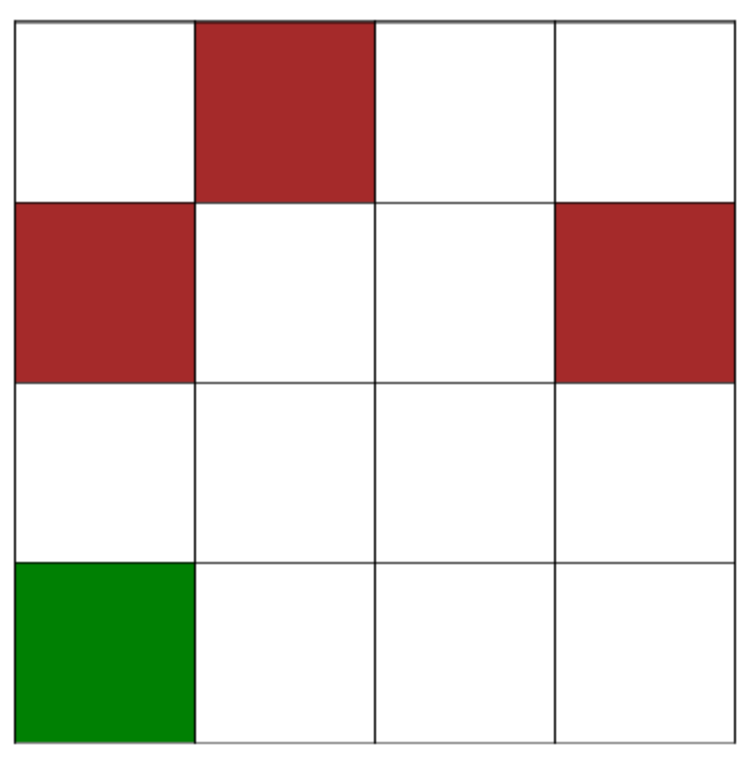
\includegraphics[width=4.5cm]{staubsauger.png}    
    \caption{Screenshot von WebTigerJython. Ein Raum mit Dreck, der gesaugt werden sollte. Was wäre hier wohl der schnellste Weg?}
\end{figure}
\section*{Regeln}
\begin{description}
    \item[Ziel:] Das Zimmer soll so effizient wie möglich gesaugt werden. Der Raum ist dann sauber, wenn Sie drei Dreck gesaugt haben.
    \item[Züge:] Ihr Roboterstaubsauger kann sich horizontal, vertikal und diagonal jeweils ein Feld bewegen.
\end{description}
\section*{Farbencodes}
\begin{description}
    \item[Grün] Die Station des Staubsaugers, die Suche beginnt hier. Sie liegt immer bei $(0,0)$
    \item[Braun] Dreck, welcher vom Staubsauger gesaugt werden sollte.
    \item[Schwarz] (Siehe optionale Aufgaben) Möbel, welche im Raum stehen und den Staubsauger behindern können.
    \item[Weiss] Freier Boden im Raum.
\end{description}


\section*{Aufgabe}
Hier werden zusätzliche Aufgaben beschrieben, welche spezifisch für Ihr Projekt sind.
Die Aufgaben sind in zwei Gruppen unterzeilt: Pflichtaufgaben und optionale Aufgaben.
Die Pflichtaufgaben sollen am Ende des Projektes beantwortet sein.
Die optionalen Aufgaben dienen dazu, sich weiter im Thema zu vertiefen.
Diese Aufgaben sind Vorschläge. Sie dürfen auch eigene Fragestellungen vertiefen.
Deklarieren Sie Ihre Fragestellungen klar im Projektbericht.
Für alle Projekt gilt natürlich, dass Sie zuerst die allgemeine Aufgabenstellung und den Code (falls vorhanden) verstehen sollten, bevor Sie die untenstehen Aufgaben bearbeiten.
\subsection*{Pflichtaufgaben}
\begin{itemize}
    \item In der Vorlage ist bereits die Tiefensuche Implementiert. Was fällt auf?
    \item Versuchen Sie für diese Problem als erstes Die Breitensuche zu implementieren. Was für Probleme ergeben sich? Ist die Lösung optimal?
    \item Reflektieren Sie, welche Regeln bezüglich Pruning für Ihr spezifisches Problem sinnvoll sind und welche nicht. Was für eine Auswirkung auf mögliche Lösungen haben die verschiedenen Pruningstrategien?
    \item Schreiben Sie ein Programm (oder verbessern Sie das existierende), welches jeweils eine optimale Lösung für Ihr Problem findet. Um dies Umzusetzen, überlegen Sie sich, was man an der Breitensuche verbessern müsste, damit Sie funktionieren würde.
\end{itemize}
\subsection*{Optionale Aufgaben}
\begin{itemize}
    \item Wie ändert sich das Problem, wenn Sie in der Konfiguration Möbel einschalten?
    \item Können Sie diese Problem mit einer Heuristik lösen? Wenn ja, welche? Wenn nicht, warum nicht?
    \item (Sehr schwierig) Recherchieren Sie den Fachbegriff \textit{Landmark Heuristik Search}. Überlegen Sie, wie Sie diese Technik in diesem Problem anwenden könnten.
\end{itemize}

\end{document}  
